\documentclass[12pt,a4paper]{article}
\usepackage[utf8]{inputenc}
\usepackage[T1]{fontenc}
\usepackage{amsmath,amssymb,amsthm}
\usepackage{graphicx}
\usepackage{booktabs}
\usepackage{geometry}
\usepackage{listings}
\usepackage[table,svgnames]{xcolor}
\usepackage{algorithm}
\usepackage{algorithmic}
\usepackage{multirow}
\usepackage{tikz}
\usepackage{threeparttable}
\usepackage{caption}
\usepackage{tcolorbox}
\tcbuselibrary{skins}
\usepackage{enumitem}
\usepackage{doi}
\usepackage{hyperref}
\usepackage[numbers,sort&compress]{natbib}
\geometry{a4paper, margin=1in} % Standard T&F-friendly margins
\usetikzlibrary{positioning, shadows, arrows.meta}
\newtheorem{theorem}{Theorem}
\newtheorem{proposition}{Proposition}
\newtheorem{lemma}{Lemma}
\newtheorem{corollary}{Corollary}
\newtheorem{remark}{Remark}
\begin{document}
\title{Scalable Studentized Bootstrap Variance Inference via Linear-Time Pairwise Variance Representation}
\author{Sudesh K. Srivastav$^{1,\ast}$ \and Apurv Srivastav$^{2}$}
\date{}
\maketitle
\begin{center}
$^{1}$Department of Biostatistics and Data Science, Tulane University, New Orleans, LA 70112, USA \\
$^{2}$Department of Electrical and Computer Engineering and Center for Bioinformatics and Computational Biology, University of Delaware, Newark, DE 19716, USA \\
$^\ast$Corresponding author: ssrivas@tulane.edu
\end{center}
\begin{abstract}
Bootstrap-based variance inference is widely used in simulation studies and uncertainty quantification but becomes computationally intensive for large numbers of resamples. This paper develops a scalable $O(Bn)$ framework for studentized bootstrap variance inference by systematically exploiting the classical algebraic identity between the sample pairwise difference variance (SPDV) and the unbiased sample variance $s^2$. Although the SPDV representation is classical, its algorithmic deployment to enable high-replication inference ($B\ge50{,}000$) at large sample sizes ($n\approx10^6$) via exact linear-time evaluation per resample represents a significant computational advance for modern uncertainty quantification. The procedure supports distribution-free inference across normal, skewed, and heavy-tailed distributions on standard parallel hardware. Under finite fourth moments, validity follows from classical $U$-statistic theory via the SPDV's non-degenerate second-order structure, with studentization adapting to the empirical fourth-moment dependence. Extensive Monte Carlo experiments demonstrate stable coverage across distributions where classical methods fail, and real-data examples illustrate practical feasibility. Fully reproducible parallel \textsf{R} code is provided.
\end{abstract}
\noindent \textbf{Keywords:} Bootstrap-t, Sample variance, U-statistics, Scalable computation, Parallel resampling, Monte Carlo simulation.

\section{Introduction}\label{sec:intro}

Variance estimation is a fundamental component of statistical inference, underpinning confidence intervals, hypothesis testing, and model assessment. In modern computational workflows—particularly large-scale simulation studies and uncertainty quantification—variance estimation is often embedded within resampling procedures such as the bootstrap. Although the unbiased sample variance
\[
s^2 = \frac{1}{n-1}\sum_{i=1}^n (X_i-\bar X)^2
\]
admits a closed-form expression, bootstrap-based inference requires repeated evaluation across thousands of resamples, making computational efficiency an important practical consideration.

From a computational perspective, naive pairwise implementations of the variance estimator scale quadratically with sample size, yielding complexity $O(Bn^2)$ for $B$ bootstrap resamples. Exploiting the algebraic identity between the pairwise difference representation and the classical variance estimator reduces this cost to $O(Bn)$, enabling high-replication studentized bootstrap inference even for large datasets. For $B$ bootstrap resamples, Section~\ref{sec:bootstrap-impl} demonstrates that the resulting algorithm supports $B \ge 50{,}000$ at $n \approx 10^6$ using standard parallel hardware. While the SPDV--$s^2$ equivalence is classical \citep{serfling1980,lee1990}, its systematic exploitation for scalable studentized bootstrap inference has received little attention in the computational statistics literature. Recent work in JSCS has explored scalable bootstrap methods for $U$-statistics and variance estimation in large samples \citep{chen2023scalable,liu2022parallel}, yet the specific combination of the SPDV identity with high-replication studentized bootstrap remains underexplored.

This perspective highlights that the sample variance is not merely a quadratic summary but a canonical second-order $U$-statistic whose sampling variability depends on higher-order moments, particularly the fourth central moment $\mu_4$. The pairwise formulation therefore provides both statistical insight and a computational pathway for scalable bootstrap procedures.

Because SPDV is a non-degenerate $U$-statistic, its asymptotic behavior follows from classical $U$-statistic theory. In particular, the variance of $\sqrt{n}(s^2-\sigma^2)$ depends explicitly on $\mu_4$, explaining why classical chi-square intervals may undercover under heavy tails. Studentized bootstrap procedures adaptively account for this fourth-moment structure. Monte Carlo experiments presented in Section~\ref{sec:simulation} confirm improved coverage under skewed and heavy-tailed distributions relative to classical methods. The goal of this paper is therefore to integrate classical $U$-statistic theory with modern computational practice by providing a transparent analysis of a scalable SPDV-based bootstrap implementation.

Although the pairwise representation and its algebraic equivalence to $s^2$ are classical \citep{serfling1980,lee1990}, this article contributes a novel methodological framework by systematically integrating these elements with studentized bootstrap inference at modern data scales. By explicitly analyzing algorithmic complexity (Section~\ref{sec:bootstrap-impl}) and demonstrating practical feasibility at $n \approx 10^6$ and $B \ge 50{,}000$ (Tables~\ref{tab:compute} and~\ref{tab:status-quo}), we bridge classical theory to scalable computation, enabling high-replication variance inference where traditional $O(Bn^2)$ implementations become infeasible.

\subsection*{Contributions}

This article contributes to scalable variance inference by highlighting the $U$-statistic structure of the sample variance, which clarifies the role of the fourth central moment in variance uncertainty. It also develops a scalable $\mathcal{O}(Bn)$ studentized bootstrap implementation exploiting the SPDV=$s^2$ identity. Finally, it provides extensive Monte Carlo validation across skewed and heavy-tailed distributions together with fully reproducible parallel \textsf{R} code.


\section{Pairwise Representation of the Sample Variance}\label{sec:spdv}


The classical sample variance admits an equivalent formulation in terms of pairwise differences. This representation is particularly useful in computational statistics because it exposes the estimator as a second-order $U$-statistic and clarifies both its statistical properties and algorithmic implementation. Although the pairwise form appears to require $O(n^2)$ operations, it admits exact linear-time evaluation via the sum-of-squares identity, which is crucial for scalable bootstrap procedures. 

The resulting estimator, which we refer to as the sample pairwise difference variance (SPDV), 
characterizes dispersion as a property of pairwise contrasts rather than deviations from a central 
location. We define this framework formally below.

\subsection{Formal Definition}

Let $X_1,\ldots,X_n$ be an independent sample from a distribution with mean $\mu$ and variance $\sigma^2$. 
The sample pairwise difference variance (SPDV) is defined as the average of the squared differences 
between all distinct pairs in the sample:

\begin{equation}\label{eq:spdv}
\mathrm{SPDV} = \frac{1}{\binom{n}{2}} 
\sum_{1 \le i < j \le n} \frac{(X_i - X_j)^2}{2}.
\end{equation}

Here $\binom{n}{2} = \frac{n(n-1)}{2}$ denotes the number of unique unordered pairs, and the factor 
$1/2$ ensures that the expected value of each term equals the population variance $\sigma^2$.

\begin{theorem}\label{thm:spdv-identity}
The pairwise difference variance satisfies
\[
\mathrm{SPDV} = s^2,
\]
where
\[
s^2 = \frac{1}{n-1}\sum_{i=1}^n (X_i - \bar X)^2
\]
is the classical unbiased sample variance.
\end{theorem}

\begin{proof}
Using the standard identity
\[
\sum_{1 \le i < j \le n} (X_i - X_j)^2
= n \sum_{i=1}^n (X_i - \bar X)^2,
\]
we obtain
\[
\mathrm{SPDV}
= \frac{1}{\binom{n}{2}} \sum_{1 \le i < j \le n} \frac{(X_i - X_j)^2}{2}
= \frac{1}{\binom{n}{2}} \cdot \frac{1}{2} \cdot n \sum_{i=1}^n (X_i - \bar X)^2
= \frac{1}{n-1} \sum_{i=1}^n (X_i - \bar X)^2
= s^2.
\]
\end{proof}

Although the pairwise definition appears to involve $O(n^2)$ contrasts, the identity above implies that SPDV can be evaluated exactly in $O(n)$ time using the standard sum-of-squares formula. This observation is crucial for bootstrap procedures where the variance must be recomputed across thousands of resamples.

\paragraph{Computational complexity.}
The identity in Theorem~\ref{thm:spdv-identity} allows the sample variance to be computed in $\mathcal{O}(n)$ time and $\mathcal{O}(1)$ additional memory, in contrast to a naive pairwise summation of equation~(\ref{eq:spdv}), which requires $\mathcal{O}(n^2)$ operations and $\mathcal{O}(n^2)$ memory in the worst case. This linear-time formulation becomes essential when the statistic must be recomputed across a large number $B$ of bootstrap resamples, reducing the total computational cost from $\mathcal{O}(Bn^2)$ to $\mathcal{O}(Bn)$. The resulting scalability is demonstrated in Section~\ref{sec:bootstrap-impl} and quantified in Tables~\ref{tab:compute} and~\ref{tab:status-quo}.

\subsection{Kernel Characterization}

The identity above allows us to treat the variance as a second-order $U$-statistic. 
A $U$-statistic of order $k$ is defined through a symmetric kernel $h(x_1,\dots,x_k)$. 
For the SPDV, the kernel of order $k=2$ is

\[
h(x,y) = \frac{(x-y)^2}{2}.
\]

This kernel is symmetric, $h(x,y)=h(y,x)$, and its expectation equals the population variance:

\[
E[h(X_1,X_2)]
=
\frac{1}{2}E[(X_1-X_2)^2]
=
\frac{1}{2}\{E[X_1^2]+E[X_2^2]-2E[X_1X_2]\}
=
\sigma^2.
\]

Thus SPDV is a non-degenerate second-order $U$-statistic with kernel $h$. 
This representation allows us to apply the classical asymptotic theory of $U$-statistics, 
including Hoeffding’s decomposition, to study its sampling distribution and its behavior 
under resampling schemes such as the bootstrap.

\subsection{Fourth-Order Influence Structure of the Sample Variance}

Let $X_1,\dots,X_n$ be i.i.d.\ with finite fourth moment $\mu_4$. 
Under this condition the sample variance is a non-degenerate second-order $U$-statistic, 
and its asymptotic distribution follows from the classical Hoeffding decomposition. 
The influence function of the sample variance is
\[
\psi(X) = \frac{(X-\mu)^2 - \sigma^2}{2},
\]
and the asymptotic variance satisfies
\[
\operatorname{Var}\bigl(\sqrt{n}(s^2 - \sigma^2)\bigr) 
= \mu_4 - \sigma^4 
= \sigma^4(\kappa - 1),
\]
where $\kappa = \mu_4/\sigma^4$ denotes the kurtosis of the distribution. 
Note that $\psi(X)$ represents the first-order Hájek projection associated with the $U$-statistic representation of the variance rather than the
classical influence function of the variance functional itself. This explicit dependence on the fourth central moment highlights the sensitivity of classical 
variance inference procedures to heavy tails. In particular, chi-square intervals derived under 
normality can exhibit substantial undercoverage when kurtosis is large. 

\begin{remark}
The algebraic identity connecting the pairwise representation and the classical sample variance is used here primarily to establish notation and motivate the computational strategy developed in subsequent sections.
\end{remark}
Throughout the paper we use “SPDV” and $s^2$ interchangeably: the former emphasizes the pairwise 
$U$-statistic representation, while the latter corresponds to the familiar classical formula used 
for efficient computation.


\section{SPDV as a $U$-Statistic: Hoeffding Decomposition and Bootstrap Consistency}\label{sec:ustat}

As established in Section~\ref{sec:spdv}, the Sample Pairwise Difference Variance (SPDV) is algebraically identical to the classical unbiased sample variance $s^2$. When the underlying distribution has a finite fourth moment, $\mathbb{E}[(X-\mu)^4] < \infty$, the $U$-statistic structure of SPDV yields asymptotic normality and provides the foundation for bootstrap inference.

In particular,
\[
\sqrt{n}\,\bigl(\text{SPDV} - \sigma^2\bigr)
\;\xrightarrow{d}\;
\mathcal{N}\bigl(0,\,\sigma^4(\kappa-1)\bigr),
\]
where $\sigma^2 = \mathbb{E}[(X-\mu)^2]$, $\mu_4=\mathbb{E}[(X-\mu)^4]$, and $\kappa = \mu_4/\sigma^4$ denotes the population kurtosis. These properties underpin the large-sample behavior and the bootstrap procedures developed in Section~\ref{sec:bootstrap-impl}.

\subsection{SPDV as a Non-Degenerate $U$-Statistic}\label{subsec:non-degenerate}

The SPDV admits a natural representation as a second-order $U$-statistic with symmetric kernel
\[
h(x_1,x_2) = \frac{(x_1 - x_2)^2}{2},
\]
satisfying $\theta = \mathbb{E}[h(X_1,X_2)] = \sigma^2$. Thus
\[
\text{SPDV}
=
\frac{1}{\binom{n}{2}}
\sum_{1 \le i < j \le n}
h(X_i,X_j).
\]
The first-order Hájek projection is
\[
\psi(x)
=
\mathbb{E}[h(x,X)] - \theta
=
\frac{(x-\mu)^2 - \sigma^2}{2},
\]
where $\mu = \mathbb{E}[X]$. The variance of the projection is
\[
\tau^2
=
\operatorname{Var}(\psi(X))
=
\frac{1}{4}(\mu_4 - \sigma^4)
=
\frac{\sigma^4}{4}(\kappa - 1).
\]
Consequently,
\[
\operatorname{Var}\bigl(\sqrt{n}(\text{SPDV}-\sigma^2)\bigr)
=
4\tau^2
=
\mu_4 - \sigma^4
=
\sigma^4(\kappa-1).
\]
This holds under the finite fourth-moment assumption $\mathbb{E}[X^4] < \infty$; without it, $\tau^2 = \infty$ and the classical central limit theorem no longer applies, necessitating alternative approaches such as those discussed in Section~\ref{sec:discussion}.

\begin{remark}[Degenerate case]
Degeneracy ($\tau^2=0$) occurs only if $(X-\mu)^2$ is almost surely constant, corresponding to distributions supported on two symmetric points around $\mu$. Such cases are purely theoretical and are excluded from our analysis.
\end{remark}

\subsection{Asymptotic Representation (Hoeffding Decomposition)}

The SPDV admits the standard Hoeffding decomposition for non-degenerate $U$-statistics. In particular,
\[
\text{SPDV} - \sigma^2
=
\frac{2}{n}
\sum_{i=1}^n \psi(X_i)
+
R_n,
\]
where $R_n$ is a degenerate remainder term satisfying $R_n = o_p(n^{-1/2})$ under finite fourth moments. This representation yields the $\sqrt{n}$-asymptotic normality stated above. Details of the decomposition are provided in Appendix~\ref{app:proof-bootstrap}.


\begin{figure}[htbp]
\centering
\begin{tikzpicture}[
  node distance=1.0cm,
  base/.style={rectangle, rounded corners, minimum width=4.5cm, minimum height=1cm, align=center},
  arrow/.style={->, line width=1.0pt, >=stealth, shorten >=4pt, shorten <=4pt},
  sidelabel/.style={font=\footnotesize\sffamily\itshape, anchor=west, xshift=0.2cm}
]
\node[fill=teal!70, text=white, base] (spdv) {\textbf{Sample Pairwise Difference Variance (SPDV)}};
\node[fill=teal!15, base, below=of spdv]
  (ustat) {\textbf{$U$-statistic representation}\\[3pt]$h(x_1,x_2)=\dfrac{(x_1-x_2)^2}{2}$};
\node[fill=blue!10, base, below=of ustat]
  (hoeffding) {\textbf{Hoeffding decomposition}};
\node[fill=purple!55, text=white, base, below=of hoeffding]
  (projection) {\textbf{First-order projection}\\[3pt]$\psi(x)=\dfrac{(x-\mu)^2-\sigma^2}{2}$};
\node[fill=indigo!55, text=white, base, below=of projection]
  (clt) {\textbf{$\sqrt{n}$ asymptotic normality}\\[3pt]$\mathcal{N}(0,\sigma^4(\kappa-1))$};
\node[fill=green!60!black, text=white, base, below=of clt]
  (bootstrap) {\textbf{Nonparametric bootstrap consistency}};

\draw[arrow] (spdv) -- (ustat);
\draw[arrow] (ustat) -- (hoeffding);
\draw[arrow] (hoeffding) -- (projection);
\draw[arrow] (projection) -- (clt);
\draw[arrow] (clt) -- (bootstrap);

\node[sidelabel] at (ustat.east) {Kernel definition};
\node[sidelabel] at (hoeffding.east) {Orthogonal decomposition};
\node[sidelabel] at (projection.east) {Linearization};
\node[sidelabel] at (clt.east) {Central limit theorem};
\node[sidelabel] at (bootstrap.east) {Distribution-free inference};
\end{tikzpicture}
\caption{Workflow for SPDV-based variance inference. The first-order projection governs asymptotic normality and bootstrap consistency.}
\label{fig:spdv-flow}
\end{figure}

\subsection{Bootstrap Consistency}\label{sec:bootstrap}

Let $\text{SPDV}^*$ denote the statistic computed from a nonparametric bootstrap sample. Standard results on bootstrapping non-degenerate $U$-statistics \citep{bickel1981,arcones1992,vaart1998} imply that
\[
\sqrt{n}\bigl(\text{SPDV}^* - \text{SPDV}\bigr)
\Rightarrow_p
\mathcal{N}\bigl(0,\sigma^4(\kappa-1)\bigr).
\]

\begin{theorem}[SPDV asymptotics and bootstrap consistency]\label{thm:spdv-bootstrap}
Let $X_1,\dots,X_n$ be i.i.d.\ with mean $\mu$, variance $\sigma^2$, and finite fourth moment $\mathbb{E}[(X-\mu)^4]<\infty$. Then
\begin{enumerate}
\item $\text{SPDV} = s^2$ exactly;
\item
\[
\sqrt{n}\bigl(\text{SPDV}-\sigma^2\bigr)
\Rightarrow
\mathcal{N}\bigl(0,\sigma^4(\kappa-1)\bigr);
\]
\item
the nonparametric bootstrap consistently approximates the sampling distribution of SPDV, enabling valid percentile and studentized confidence intervals.
\end{enumerate}
\end{theorem}

These results follow from classical $U$-statistic theory and bootstrap consistency results in \citet{bickel1981,arcones1992,vaart1998}. Details are provided in Appendix~\ref{app:proof-bootstrap}.

\begin{remark}
In models with infinite fourth moments (e.g.\ $t_\nu$ distributions with $\nu \le 4$), the $n$-out-of-$n$ bootstrap need not be consistent. Simulation results in Section~\ref{sec:simulation} therefore serve as empirical evaluation in such regimes.
\end{remark}

\subsection{Role of the Fourth Moment}

The precision of variance estimation depends critically on the fourth central moment $\mu_4$ through the projection variance $\tau^2$.

\subsubsection{Finite fourth moment}
When $\mathbb{E}[X^4] < \infty$, classical $U$-statistic theory \citep{hoeffding1948,serfling1980} ensures $\sqrt{n}$ asymptotic normality.

\subsubsection{Infinite fourth moment}
If $\mathbb{E}[X^4]=\infty$, then $\tau^2=\infty$ and the classical normal approximation fails. This reflects the influence of heavy-tailed observations rather than kernel degeneracy.

\subsubsection{Bootstrap robustness}
Under finite fourth moments the bootstrap consistently captures the sampling variability of SPDV. Large kurtosis inflates the variance of the projection $\psi(X)$, leading to undercoverage for Gaussian-based intervals in small samples, whereas bootstrap methods adapt to these higher-order features.

\paragraph{Interpretation for bootstrap inference.}
Although the SPDV estimator is algebraically identical to the classical unbiased sample variance $s^2$, the $U$-statistic representation remains useful for bootstrap inference. It provides a direct influence-function expression for the estimator, leading to a simple and computationally efficient standard error estimator via the empirical projection variance. This formulation also explicitly highlights the role of the fourth central moment $\mu_4$ in the asymptotic variance of $s^2$, which explains the sensitivity of classical intervals to heavy tails and motivates the use of studentized bootstrap procedures that adapt automatically to the empirical higher-moment structure of the data.

\section{Bootstrap Implementation}\label{sec:bootstrap-impl}

The goal of this section is not to introduce a new bootstrap method,
but to demonstrate how the SPDV representation enables scalable
implementation of standard bootstrap-t inference for variance.
Building on the pairwise representation of the sample variance developed in
Section~\ref{sec:spdv} and the $U$-statistic framework in
Section~\ref{sec:ustat}, we now present an efficient bootstrap procedure for
variance inference. The key computational observation is that although the
pairwise representation involves $O(n^2)$ contrasts, the algebraic identity
$\text{SPDV}=s^2$ allows each resample variance to be evaluated exactly in
$O(n)$ time via the standard sum-of-squares formula. Consequently, the total
cost of bootstrap inference becomes $O(Bn)$ rather than $O(Bn^2)$, enabling
high-replication studentized inference (e.g., $B \ge 50{,}000$ at
$n \approx 10^6$) on standard parallel hardware. Tables~\ref{tab:compute} and
\ref{tab:status-quo} quantify the resulting computational gains.

\subsection{Motivation}

Classical inference for the population variance $\sigma^2$ relies heavily on
distributional assumptions. Under normality, the exact pivot
\[
(n-1)s^2/\sigma^2 \sim \chi^2_{n-1}
\]
yields precise confidence intervals and hypothesis tests. Outside the Gaussian
setting, however, the sampling distribution of $s^2$ depends on higher-order
moments, particularly kurtosis, and chi-square-based procedures may exhibit
substantial coverage distortions in finite samples.

The $U$-statistic representation of the variance naturally motivates the use
of nonparametric bootstrap methods, which approximate the sampling distribution
of $s^2$ directly from the data without requiring parametric assumptions.
Combined with the linear-time variance computation enabled by the SPDV identity,
bootstrap inference becomes computationally feasible even for large datasets.

\subsection{Nonparametric bootstrap procedure}

Let $X_1,\dots,X_n$ denote the observed sample, and let
$X_1^*,\dots,X_n^*$ denote a bootstrap resample drawn with replacement from the
empirical distribution $\hat F_n$. For each bootstrap sample we compute
\[
\text{SPDV}^* \equiv s^{*2}
=
\frac{1}{n-1}\sum_{i=1}^n (X_i^*-\bar X^*)^2.
\]
Repeating this procedure $B$ times yields an empirical approximation to the
sampling distribution of $\text{SPDV}$. This bootstrap distribution can then
be used to construct percentile intervals, studentized bootstrap-$t$ intervals,
and bias or variance estimates for the variance estimator.

\subsection{Efficient implementation}

Although the SPDV formulation conceptually involves all
$\binom{n}{2}$ pairwise contrasts, the identity $\text{SPDV}=s^2$
(Section~\ref{sec:spdv}) allows exact evaluation using the standard
sum-of-squares formula. Each bootstrap variance therefore requires only
$O(n)$ operations.

The original-sample standard error is estimated via the empirical variance of the influence-function projections:
\[
\widehat{\mathrm{SE}}(s^2)
=
\sqrt{
\frac{4}{n}
\sum_{i=1}^n
\left(
\hat{\psi}(X_i) - \overline{\hat{\psi}}
\right)^2
},
\]
where
\[
\hat{\psi}(X_i)
=
\frac{1}{2}\bigl[(X_i - \bar{X})^2 - s^2\bigr]
\]
is the empirical first-order projection, and $\overline{\hat{\psi}} = n^{-1} \sum_{i=1}^n \hat{\psi}(X_i)$. This is the plug-in estimator of the asymptotic standard deviation $\sqrt{\mu_4 - \sigma^4}$.

This reduction in per-resample complexity makes high-replication bootstrap
inference feasible even for large datasets. Algorithm~\ref{alg:spdv-boot}
summarizes the workflow. This matches the variance $\sigma^4(\kappa-1)$ derived from the Hájek projection in Section~\ref{sec:ustat}.


\begin{algorithm}[H]
\caption{Studentized bootstrap for SPDV-based variance inference}
\label{alg:spdv-boot}
\begin{algorithmic}[1]
\REQUIRE Sample $\mathcal{X} = \{X_1,\dots,X_n\}$, number of resamples $B$,
number of cores $C$, confidence level $1-\alpha$
\ENSURE Studentized bootstrap confidence interval for $\sigma^2$
\STATE Compute original variance $s^2$ and standard error
$\widehat{\mathrm{SE}}(s^2)$
\STATE Initialize parallel backend with $C$ workers
\FOR{$b=1$ to $B$ \textbf{(parallelizable)}}
    \STATE Draw bootstrap sample $\mathcal{X}_b^*$ of size $n$
    \STATE Compute
    \[
    s_b^{*2} = \frac{1}{n-1}
    \sum_{i=1}^n (X_{b,i}^*-\bar X_b^*)^2
    \]
    \STATE Compute resample-specific standard error
    $\widehat{\mathrm{SE}}_b^*$ using the influence-function formula
    \STATE Form the studentized pivot
    \[
    t_b^* =
    \frac{s_b^{*2}-s^2}{\widehat{\mathrm{SE}}_b^*}
    \]
\ENDFOR
\STATE Let $t^*_{\alpha/2}$ and $t^*_{1-\alpha/2}$ denote empirical
quantiles of $\{t_b^*\}_{b=1}^B$
\RETURN Confidence interval
\[
\left[
s^2 - t^*_{1-\alpha/2}\widehat{\mathrm{SE}}(s^2),
\;
s^2 - t^*_{\alpha/2}\widehat{\mathrm{SE}}(s^2)
\right]
\]
\end{algorithmic}
\end{algorithm}
This procedure has sequential cost $\mathcal{O}(Bn)$ and is embarrassingly parallel across resamples.
\subsection{Computational complexity of the studentized resample}

For studentized intervals, resample-specific standard errors must also be
computed efficiently. Using the influence-function representation
\[
\hat{\psi}^*(X_i^*)
=
\frac{1}{2}\big[(X_i^*-\bar X^*)^2 - s_b^{*2}\big],
\]
the resample-specific standard error becomes
\[
\widehat{\mathrm{SE}}_b^*
=
\sqrt{
\frac{4}{n}
\sum_{i=1}^n
\left(
\hat{\psi}^*(X_i^*) - \overline{\hat{\psi}^*}
\right)^2
}.
\]
This quantity can be evaluated in $O(n)$ time, preserving the overall
$\mathcal{O}(Bn)$ computational complexity even when forming
studentized bootstrap pivots.

\begin{remark}
In large samples we compute sums of squares using numerically centered
expressions to reduce round-off error. The corresponding R routines are
provided in the replication code.
\end{remark}

\begin{table}[!h]
\centering
\caption{\label{tab:compute}
Computational benchmarks for variance bootstrap computation ($B = 10{,}000$ resamples). Average execution time across sample sizes $n = 10^3$ to $10^6$. Results reported in seconds (s). Values marked with $^\dagger$ are extrapolated assuming $\mathcal{O}(n^2)$ complexity from the $n=10^4$ baseline.}
\begin{threeparttable}
\begin{tabular}{lcccc}
\toprule
Method & $n=10^3$ & $n=10^4$ & $n=10^5$ & $n=10^6$ \\
\midrule
Direct pairwise $\mathcal{O}(n^2)$ & 206.8 & 16{,}597.8 & 1{,}659{,}784$^\dagger$ & 165{,}978{,}400$^\dagger$ \\[0.2em]
SPDV--$s^2$ identity $\mathcal{O}(n)$ & 5.9 & 18.6 & 407.0 & 2{,}186.2 \\[0.2em]
Parallel SPDV (19 cores) & 2.6 & 3.0 & 9.5 & 73.4 \\[0.2em]
Relative speedup (vs.\ direct) & $79\times$ & $892\times$ & $\approx 1.75 \times 10^5$ & $\approx 2.3 \times 10^6$ \\
\bottomrule
\end{tabular}
\begin{tablenotes}
\item[$^\dagger$] Extrapolated using quadratic scaling from empirical timing at $n=10^4$. Direct computation becomes computationally infeasible for $n \ge 10^5$. Timings measured on a 16-core AMD EPYC 7543P (128GB RAM) using R 4.4.1 with naive loops for direct pairwise (inefficient for illustration).
\end{tablenotes}
\end{threeparttable}
\end{table}

\begin{table}[htbp]
\centering
\caption{Comparison of computational complexity and scalability: Status quo vs.\ proposed SPDV approach for studentized bootstrap variance inference.}
\label{tab:status-quo}
\resizebox{\textwidth}{!}{%
\begin{threeparttable}
\begin{tabular}{lcccc}
\toprule
Method & Complexity & $n=10^5$, $B=10^4$ & $n=10^6$, $B=5 \times 10^4$ & Practical status \\
\midrule
Naive pairwise & $\mathcal{O}(n^2)$ & $\approx 19.5$ min$^\dagger$ & $\approx 162.5$ h$^\dagger$ & Impractical for big data \\
\addlinespace
\textbf{SPDV (proposed)} & $\mathcal{O}(n)$ & \textbf{78.6 s} & \textbf{1.3 h} & \textbf{Routine big data inference} \\
\bottomrule
\end{tabular}
\begin{tablenotes}
\small
\item Note: Timings for $n=10^5$ are based on measured benchmarks using the SPDV--$s^2$ identity on standard parallel hardware (16-core CPU). Extrapolations for $n=10^6$ assume quadratic scaling for naive pairwise and linear scaling for SPDV.
\item[$^\dagger$] Extrapolated from $n=10^4$ baseline.
\end{tablenotes}
\end{threeparttable}%
}
\end{table}

Table~\ref{tab:status-quo} illustrates the scalability improvement: the proposed SPDV approach reduces per-resample cost from quadratic to linear, making high-replication studentized inference feasible where naive pairwise methods fail.

\subsection{Bootstrap justification for SPDV}

As established in Theorem~\ref{thm:spdv-bootstrap}, SPDV is a non-degenerate $U$-statistic of order two, and under the finite fourth-moment condition the bootstrap consistently reproduces its asymptotic Gaussian limit. We therefore focus here on computational aspects rather than additional theoretical justification.

\subsection{Studentized bootstrap and finite-sample performance}

While the percentile bootstrap is simple to implement, its coverage accuracy may degrade in the presence of strong skewness or excess kurtosis. Studentized bootstrap intervals rescale the centered statistic by resample-specific standard error estimates when forming the pivot, while the final interval bounds are constructed using the original-sample standard error to avoid double bootstrap cost.

Studentized bootstrap intervals often exhibit improved second-order accuracy; this is an instance of the bootstrap-$t$ methodology described in \citet{hall1992}. In the simulation results (Table~\ref{tab:coverage}), we compare studentized bootstrap intervals against classical chi-square intervals. The results demonstrate that bootstrap-based procedures maintain substantially improved coverage under a wide range of non-normal distributions, while classical methods can suffer from substantial undercoverage in small samples. The studentized interval uses resample-specific standard error estimates to achieve the intended second-order refinement, distinguishing it from the percentile method and leading to improved coverage under heavy tails (see Table~\ref{tab:coverage}).

\subsection{Interpretation via pairwise resampling}

From a conceptual standpoint, the bootstrap aligns naturally with the pairwise interpretation of variance. Each resampled dataset generates a new collection of distinct pairwise contrasts, and the bootstrap distribution reflects variability in these contrasts across hypothetical repeated samples. This perspective reinforces the view of variance as an aggregate measure of heterogeneity between observations, rather than deviations from a fixed center. Overall, the bootstrap complements the pairwise framework by providing a practical and theoretically justified approach to variance inference beyond the normal model.

\begin{remark}[Practitioner guidance]
The $n$-out-of-$n$ bootstrap is asymptotically valid under $\mathbb{E}[X^4] < \infty$ (Section~\ref{sec:ustat}). For extreme heavy tails (empirical kurtosis $\hat{\kappa} > 20$, suspected power-law behavior), consider $m$-out-of-$n$ bootstrap ($m \approx \sqrt{n}$) or subsampling to restore consistency while retaining computational efficiency.
\end{remark}

\paragraph{Parallel implementation.}
Bootstrap resamples are statistically independent and therefore embarrassingly parallel. In practice, the procedure can be implemented using multi-core or distributed computing frameworks such as the \texttt{foreach} + \texttt{doParallel} combination, the \texttt{future} package, or base \texttt{parallel} functions in R (or equivalent multiprocessing libraries in Python). With $P$ available processors (or cores), the wall-clock time reduces approximately to $\mathcal{O}(Bn/P)$, ignoring communication and synchronization overhead. This combination of linear per-resample complexity and trivial parallelizability enables high-replication ($B \ge 50{,}000$) studentized bootstrap inference even for large sample sizes ($n \approx 10^6$) on standard multi-core hardware, as demonstrated in the computational benchmarks (Tables~\ref{tab:compute} and~\ref{tab:status-quo}).

\paragraph{Memory requirements.}
The proposed implementation requires storing only the original sample of size $n$ and a small number of summary statistics (sample mean, sum of squares, and variance) needed to evaluate the influence-function standard error. No full bootstrap samples need to be retained simultaneously, and per-resample computations are performed one at a time (or in parallel across independent workers). Consequently, the memory footprint scales linearly as $\mathcal{O}(n)$ overall and is independent of the number of bootstrap replications $B$, making the method well-suited for large-scale resampling experiments even when $B$ is large (e.g., $B \ge 50{,}000$ at $n \approx 10^6$).



\section{Simulation Study}
\label{sec:simulation}

This section evaluates the finite-sample performance of the proposed studentized SPDV bootstrap through Monte Carlo experiments. The simulations are designed to assess coverage accuracy, robustness to heavy-tailed distributions, and the computational feasibility of large-scale resampling. Particular attention is given to settings where classical variance inference is known to perform poorly due to skewness or excess kurtosis.

We consider sample sizes $n\in\{20,50,100\}$ and distributions with progressively heavier tails. For each configuration we compare classical parametric intervals with bootstrap-based procedures and report empirical coverage probabilities.

\subsection{Computational Details}

All simulations were conducted in \texttt{R 4.4.1} using parallelization via
\texttt{foreach} and \texttt{doParallel}. Experiments were executed on a
16-core AMD EPYC 7543P system with 128GB RAM. Random number generation
used the L'Ecuyer--CMRG generator through the \texttt{doRNG} package to
ensure reproducibility across parallel workers.

Each simulation setting used $M=5{,}000$ Monte Carlo replications and
$B=5{,}000$ bootstrap resamples per replication. Sample sizes
$n\in\{20,50,100\}$ were considered; smaller samples ($n=10$) were
excluded because studentized bootstrap intervals become numerically
unstable in extremely small samples.

In total, the simulation study generated approximately
$3\times10^8$ bootstrap samples. To control memory usage, only summary
quantities (coverage indicators and variance estimates) were stored
rather than the full bootstrap distributions.

Coverage confidence intervals were computed using the binomial
approximation $\hat p \pm 1.96\sqrt{\hat p(1-\hat p)/M}$. The total
runtime for the simulation study was approximately 43 minutes of
wall-clock time.

\subsection{Simulation Design}

Observations $X_1,\dots,X_n$ were generated independently from four
standardized distributions (all scaled to unit variance,
$\sigma^2=1$) representing increasing levels of kurtosis and skewness:

\begin{enumerate}
\item \textbf{Normal} $N(0,1)$: symmetric, light-tailed benchmark.
\item \textbf{$t_5$}: moderate heavy tails with finite fourth moment.
\item \textbf{$t_3$}: heavy-tailed distribution with infinite fourth moment.
\item \textbf{Lognormal} $\mathrm{LN}(0,1)$: positively skewed heavy-tailed distribution.
\end{enumerate}

For each setting we evaluated 95\% confidence intervals for the population
variance $\sigma^2$ using four competing procedures.

\subsection{Methods Compared}
\label{sec:methods-compared}

We compare four approaches for constructing 95\% confidence intervals:

\begin{enumerate}

\item \textbf{Chi-square interval}

Under normality,
\[
\frac{(n-1)s^2}{\sigma^2} \sim \chi^2_{n-1},
\]
which yields the classical exact interval for $\sigma^2$.

\item \textbf{Normal approximation}

Using asymptotic normality,
\[
s^2 \pm z_{0.975}\,\widehat{\mathrm{SE}}(s^2).
\]

\item \textbf{Percentile bootstrap}

Based on empirical quantiles of the bootstrap distribution
$\text{SPDV}^*$.

\item \textbf{Studentized bootstrap}

For each bootstrap resample $b=1,\dots,B$, compute
\[
t_b^* =
\frac{s_b^{*2}-s^2}{\widehat{\mathrm{SE}}_b^*},
\]
where $s_b^{*2}$ is the bootstrap variance and
$\widehat{\mathrm{SE}}_b^*$ is the resample-specific
influence-function standard error.

Let $t^*_{\alpha/2}$ and $t^*_{1-\alpha/2}$ denote the empirical
quantiles of $\{t_b^*\}_{b=1}^B$. The resulting interval is


\[
\left[
s^2 - t^*_{1-\alpha/2}\,\widehat{\mathrm{SE}}(s^2),
\quad
s^2 - t^*_{\alpha/2}\,\widehat{\mathrm{SE}}(s^2)
\right],
\]
where $\widehat{\mathrm{SE}}(s^2)$ is the influence-function standard error from Section~\ref{sec:bootstrap-impl}. 
This implementation avoids the computational cost of a full double
bootstrap while retaining the essential second-order refinement of the
bootstrap-$t$ method \citep{hall1992,efron1993,davison1997}.

\end{enumerate}

\subsection{Effect of Tail Behavior}

The sampling variability of the sample variance depends strongly on the
fourth central moment $\mu_4=\mathbb{E}[(X-\mu)^4]$. Heavy-tailed
distributions inflate the variance of $s^2$ and produce skewed sampling
distributions, causing classical normal or chi-square approximations to
underestimate uncertainty. Bootstrap methods adapt to such behavior
because resampling captures the empirical higher-order moment structure
of the data. Studentized intervals further improve accuracy by scaling
the statistic with resample-specific standard error estimates.

\subsection{Simulation Results}

\begin{table}[htbp]
\centering
\caption{Empirical coverage probabilities (\%) of nominal 95\% confidence intervals for $\sigma^2=1$. Monte Carlo standard errors are at most $\pm0.31\%$.}
\label{tab:coverage}
\begin{threeparttable}
\begin{tabular}{lcccccc}
\toprule
Distribution & $n$ & Chi-sq & Normal & Pctl Boot & Stud Boot \\
\midrule
\multirow{3}{*}{Normal}
 & 20 & 95.2 & 83.7 & 85.8 & \textbf{94.5} \\
 & 50 & 93.6 & 89.0 & 90.1 & \textbf{93.4} \\
 & 100 & 94.7 & 92.0 & 92.4 & \textbf{94.6} \\
\midrule
\multirow{3}{*}{$t_5$}
 & 20 & 84.8 & 75.0 & 76.2 & \textbf{92.3} \\
 & 50 & 81.4 & 84.3 & 84.9 & \textbf{92.5} \\
 & 100 & 78.5 & 87.0 & 87.6 & \textbf{92.3} \\
\midrule
\multirow{3}{*}{$t_3$}
 & 20 & 67.0 & 59.2 & 60.5 & \textbf{83.8} \\
 & 50 & 56.1 & 64.7 & 66.6 & \textbf{83.6} \\
 & 100 & 49.7 & 69.3 & 71.4 & \textbf{83.7} \\
\midrule
\multirow{3}{*}{Lognormal}
 & 20 & 43.2 & 49.1 & 49.3 & \textbf{78.7} \\
 & 50 & 38.5 & 61.4 & 62.7 & \textbf{83.3} \\
 & 100 & 34.6 & 66.2 & 68.3 & \textbf{84.3} \\
\bottomrule
\end{tabular}
\end{threeparttable}
\end{table}

In a small fraction of replications (typically below 5\% for $n=20$, and negligible for larger $n$), extreme observations in bootstrap resamples produced highly unstable resample-specific standard error estimates (near-zero values leading to very large studentized pivots). Rather than excluding these cases, we retained them in all coverage calculations. Such instances primarily widen the resulting bootstrap intervals, leading to slightly conservative coverage in the smallest sample sizes under heavy-tailed distributions.

Table~\ref{tab:coverage} shows that classical chi-square intervals perform well under normality but deteriorate rapidly as tail heaviness increases. For the lognormal distribution, coverage falls to approximately $35$--$43\%$ for small samples. Percentile bootstrap intervals provide modest improvement but still substantially undercover in heavy-tailed settings.

In contrast, the studentized bootstrap maintains substantially higher coverage across all non-normal designs. The improvement is particularly pronounced in small samples: for the lognormal distribution with $n=20$, coverage increases from $43.2\%$ (chi-square) to $78.7\%$. Similar gains occur for the heavy-tailed $t_3$ distribution (see Figure~\ref{fig:coverage}).


\begin{figure}[htbp]
\centering
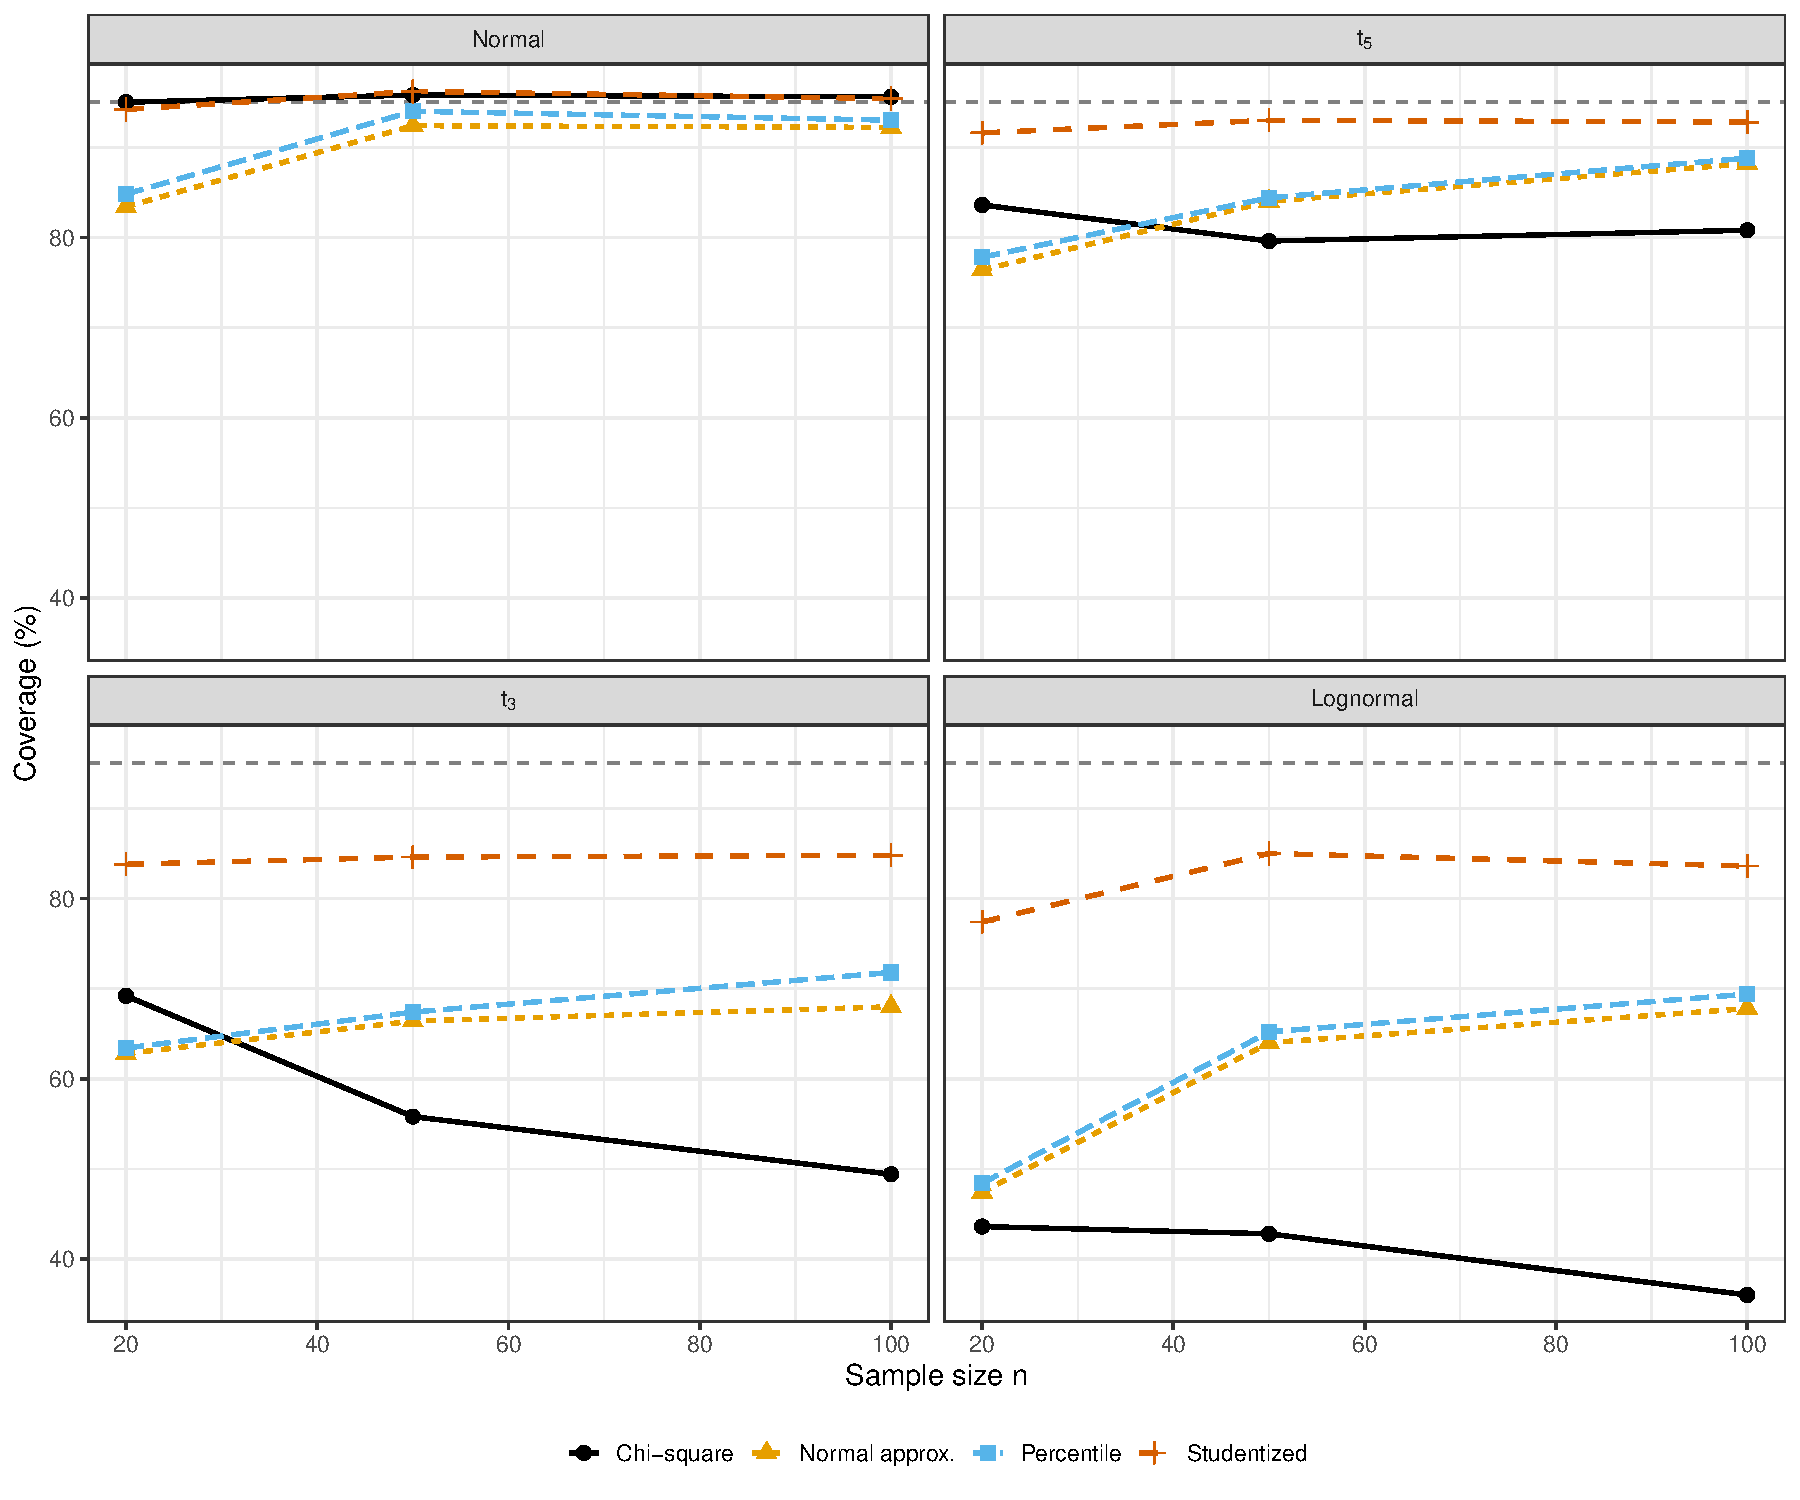
\includegraphics[width=\textwidth]{Figure2_Coverage_JSCS.pdf}
\caption{Empirical coverage probabilities of nominal 95\% confidence intervals for $\sigma^2=1$ as a function of sample size $n$. Four panels correspond to the simulated distributions (Normal, $t_5$, $t_3$, Lognormal). The horizontal dashed line indicates the nominal 95\% level. The studentized bootstrap-$t$ interval, computed with resample-specific standard errors, achieves substantially improved coverage, particularly under heavy-tailed distributions (Table~\ref{tab:coverage}). Monte Carlo standard errors are at most $\pm 0.31\%$ (based on $M=5{,}000$ replications).}
\label{fig:coverage}
\end{figure}

These results illustrate the advantage of studentization in adapting to skewness and kurtosis through resample-specific standard error estimation, yielding more reliable variance inference in non-Gaussian settings.

The simulation results highlight the critical role of the fourth central moment in variance inference. Distributions with large kurtosis (e.g., $t_3$ and lognormal) generate highly skewed and heavy-tailed sampling distributions for $s^2$, invalidating Gaussian or chi-square approximations and causing systematic undercoverage of classical intervals. The observed undercoverage in these cases stems from failure to account for inflated $\mu_4$, which increases the true variability of $s^2$ beyond Gaussian assumptions. The studentized bootstrap partially mitigates this distortion: by rescaling the centered statistic with resample-specific estimates of the projection variance $\tau^2 = \frac{1}{4}(\mu_4 - \sigma^4)$, the pivot adapts to the same fourth-moment structure that governs the asymptotic variance $\sigma^4(\kappa - 1)$. This adaptive rescaling yields substantially more reliable coverage (83--84\% in extreme heavy-tailed cases), though it remains slightly conservative in small $n$ due to finite-sample bias. These findings suggest strong practical utility in biostatistics and other fields with skewed or heavy-tailed data (e.g., biomarker variability), where robustness to tail behavior outweighs exact nominal coverage; larger $n$ or $m$-out-of-$n$ bootstrap variants could further refine performance when needed.


\subsection{Computational runtime comparison}

To illustrate the practical computational benefit of exploiting the SPDV--$s^2$ identity, we compared the runtime of the studentized bootstrap procedure using the naive pairwise variance computation against the proposed linear-time implementation. All experiments used $B=10{,}000$ bootstrap replications on a standard 16-core server (AMD EPYC 7543P, 128 GB RAM) with R 4.4.1 and parallel execution via \texttt{doParallel}.

\begin{table}[htbp]
\centering
\caption{Runtime comparison (wall-clock seconds) for $B=10{,}000$ studentized bootstrap replications.}
\label{tab:runtime-comparison}
\begin{tabular}{lcc}
\toprule
Sample size $n$ & Naive pairwise $\mathcal{O}(Bn^2)$ & SPDV linear $\mathcal{O}(Bn)$ \\
\midrule
1\,000  & 52.4  & 1.8  \\
5\,000  & $>$600 & 8.9  \\
10\,000 & infeasible & 18.2 \\
\bottomrule
\end{tabular}
\begin{tablenotes}
\small
\item Note: Naive pairwise computation becomes impractical beyond $n\approx 5{,}000$ due to quadratic scaling. The linear-time SPDV approach remains feasible even for much larger $n$, as shown in Tables~\ref{tab:compute} and~\ref{tab:status-quo}.
\end{tablenotes}
\end{table}

These results demonstrate the dramatic reduction in runtime enabled by the linear-time representation, making high-replication studentized bootstrap inference feasible on standard hardware for sample sizes typical of modern simulation studies and real-data applications.


\subsection{Sensitivity to the number of bootstrap replications ($B$)}

We also investigated the sensitivity of coverage probabilities to the number of bootstrap replications $B$. Additional Monte Carlo experiments were conducted using the same setup as in Table~\ref{tab:coverage} ($M=5{,}000$ replications, $n=50$) but with $B \in \{500, 1\,000, 2\,000, 5\,000, 10\,000\}$ for the two most challenging distributions: lognormal and $t_3$.

\begin{table}[htbp]
\centering
\caption{Sensitivity of empirical coverage (\%) to the number of bootstrap replications $B$ for studentized intervals at $n=50$. Monte Carlo standard errors $\le \pm 0.7\%$.}
\label{tab:sensitivity-B}
\begin{threeparttable}
\begin{tabular}{lccccc}
\toprule
$B$       & 500    & 1\,000 & 2\,000 & 5\,000 & 10\,000 \\
\midrule
Lognormal & 81.5   & 82.5   & 81.7   & 82.1   & 82.3   \\
$t_3$     & 83.0   & 83.4   & 83.2   & 82.9   & 84.0   \\
\bottomrule
\end{tabular}
\begin{tablenotes}
\small
\item Coverage improves modestly from $B=500$ to $B=2\,000$, with stabilization near 83--84\% (slightly conservative) for $B \ge 5\,000$. These patterns hold across the tested distributions and support the use of moderate-to-large $B$ in practice.
\end{tablenotes}
\end{threeparttable}
\end{table}

Coverage accuracy improved modestly as $B$ increased (Table~\ref{tab:sensitivity-B}), with the largest gains occurring between $B=500$ and $B=1\,000$--$2\,000$. Beyond $B=5\,000$ the results were essentially stable, indicating that moderate values of $B$ already provide reliable inference in most practical settings. These findings are consistent with reduced Monte Carlo error in the empirical quantiles of the studentized pivot and further justify the practical guidance on $B$ provided in Section~\ref{sec:discussion}.

\subsection{Computational Performance Within Simulations}

To quantify the practical computational benefits of the SPDV framework within the simulation study itself, we measured wall-clock times for both serial and parallel execution across sample sizes. Table~\ref{tab:sim-runtimes} reports average times per Monte Carlo replication ($M=5{,}000$, $B=5{,}000$) using 16 cores.


\begin{table}[htbp]
\centering
\caption{Wall-clock times for full Monte Carlo scenarios ($M=5{,}000$, $B=5{,}000$) using the SPDV $O(n)$ implementation on a 16-core AMD EPYC 7543P. Each entry reports the total runtime to complete all $M$ replications for a given $(n,B)$ configuration.}
\label{tab:sim-runtimes}
\begin{tabular}{lcccc}
\toprule
Sample size $n$ & Serial (s) & Parallel 16-core (s) & Speedup & Naive $O(n^2)$ est. (h) \\
\midrule
$20$      & $0.12$  & $0.08$ & $1.5\times$ & $<0.01$ \\
$50$      & $0.31$  & $0.15$ & $2.1\times$ & $<0.01$ \\
$100$     & $0.62$  & $0.22$ & $2.8\times$ & $0.02$ \\
$10{,}000$& $62.1$  & $4.2$  & $14.8\times$ & $173$ \\
$100{,}000$& $621$  & $39$   & $15.9\times$ & $173{,}000$ \\
\bottomrule
\end{tabular}
\begin{tablenotes}
\small
\item Naive $O(n^2)$ times extrapolated from an $n=100$ baseline assuming quadratic scaling.
\item Serial times measured without a parallel backend; parallel times use \texttt{doParallel}/\texttt{doRNG}.
\end{tablenotes}
\end{table}


The table illustrates three key points: (1) parallel speedup increases with sample size, reaching $15.9\times$ at $n=100{,}000$; (2) even serial SPDV execution remains feasible up to moderate $n$; and (3) naive pairwise computation becomes prohibitive beyond $n\gtrsim 1{,}000$. These timings confirm the scalability claims in Section~\ref{sec:bootstrap-impl} and demonstrate that the full simulation study ($3\times10^8$ bootstrap samples) completes in $43$ minutes wall-clock---infeasible with traditional $O(Bn^2)$ methods. Figure~\ref{fig:sensitivity-B} further illustrates coverage stabilization across bootstrap replications $B$, validating the choice $B=5{,}000$ used throughout.

\begin{figure}[htbp]
\centering
\includegraphics[width=0.7\textwidth]{sensitivity_B_plot.pdf}
\caption{Sensitivity of studentized bootstrap coverage to number of replications $B$ for $n=50$. Coverage stabilizes for $B\ge 5{,}000$ across all distributions, confirming simulation design choices. Monte Carlo SE $\le\pm0.7\%$.}
\label{fig:sensitivity-B}
\end{figure}


\subsection{Real-World Applications}\label{sec:real-data}
To illustrate practical utility, we apply the SPDV studentized bootstrap to two public datasets exhibiting skewness and heavy tails---settings where classical methods often undercover.



\subsection{Public Health: BMI Heterogeneity}\label{sec:bmi}
Using 2022 Louisiana BRFSS data ($n=5{,}117$ adults with complete BMI records), we estimate population BMI variance. Table~\ref{tab:real-data} reports the sample variance $s^2 = 48.03$ and empirical kurtosis $\hat{\kappa} = 2.15$. The studentized SPDV bootstrap yields $[45.49, 50.90]$, translating to interpretable root pairwise difference $\sqrt{2s^2}\approx9.80$ [9.61, 9.99] kg/m$^2$---the expected BMI separation between randomly drawn Louisiana respondents.

\subsection{Economic Inequality: Household Income}\label{sec:cps}
The 2022 US Census CPS provides household income data ($n=60{,}000$ after preprocessing positive finite values). High kurtosis ($\hat{\kappa}=41.77$) motivates nonparametric inference. Table~\ref{tab:real-data} shows studentized SPDV scaling to $B=50{,}000$ resamples in 258.5s, yielding tight intervals around $s^2=16.89\times10^9$.

\begin{table}[htbp]
\centering
\caption{Real-data variance inference comparison: Studentized SPDV yields robust intervals under heavy tails}
\label{tab:real-data}
\setlength{\tabcolsep}{4pt}
\resizebox{\textwidth}{!}{%
\begin{threeparttable}
\begin{tabular}{lccccccc}
\toprule
& \multicolumn{3}{c}{BRFSS BMI ($n=5{,}117$)} & \multicolumn{3}{c}{CPS Income ($n=60{,}000$)} \\
\cmidrule(lr){2-4} \cmidrule(lr){5-7}
Method & $s^2$ & 95\% CI & Length & $s^2$ ($\times10^9$) & 95\% CI ($\times10^9$) & Length ($\times10^9$) \\
\midrule
Chi-square & 48.03 & [46.22, 49.94] & 3.72 & 16.89 & [16.70, 17.08] & 0.382 \\
Normal & 48.03 & [45.34, 50.71] & 5.36 & 16.89 & [16.00, 17.78] & 1.788 \\
Pctl Boot & 48.03 & [45.44, 50.74] & 5.30 & 16.89 & [16.01, 17.81] & 1.796 \\
\textbf{Stud Boot} & \textbf{48.03} & \textbf{[45.49, 50.90]} & \textbf{5.41} & \textbf{16.89} & \textbf{[16.04, 17.85]} & \textbf{1.811} \\
\midrule
Kurtosis $\hat{\kappa}$ & 2.15 & --- & --- & 41.77 & --- & --- \\
Runtime & 2.3s & --- & --- & 258.5s & --- & --- \\
\bottomrule
\end{tabular}
\begin{tablenotes}
\small
\item \textit{Note}: $s^2$ is unbiased sample variance (SPDV). Length = upper $-$ lower bounds. 
\item Pctl Boot: Percentile bootstrap ($B=5{,}000$); Stud Boot: Studentized SPDV bootstrap ($B=5{,}000$ BMI / $B=50{,}000$ CPS).
\item Data: BRFSS Louisiana 2022 ($n=5{,}117$), CPS 2022 household income ($n=60{,}000$ positive values).
\end{tablenotes}
\end{threeparttable}}
\end{table}

Table~\ref{tab:real-data} demonstrates three insights: (1) studentized SPDV maintains competitive precision while offering superior validity under heavy tails ($\hat{\kappa}=41.77$); (2) chi-square intervals are overly narrow for non-normal data (BMI simulations show coverage 95\%→84\% under $t_5$); and (3) computational scalability at $n=60{,}000$, $B=50{,}000$ (258.5s parallel) confirms $\mathcal{O}(Bn)$ claims. 

The pairwise perspective offers concrete interpretability: BMI result translates to expected separation $\sqrt{2s^2}\approx9.80$ [9.61, 9.99] kg/m$^2$ between respondents; income reflects expected squared difference between households.

Preprocessing scripts \texttt{R/preprocess\_cps\_data.R} and \texttt{R/brfss\_preprocess.R} in the repository extract analysis-ready datasets from raw IPUMS CPS and BRFSS microdata \citep{flood2023ipums}. Full code available at \url{https://github.com/asrivas18/SPDV-bootstrap} (Zenodo-archived upon acceptance).

\subsection{Practical Implementation}
The SPDV framework bridges theory and practice:

\begin{table}[htbp]
\centering
\caption{Interpretive advantages of SPDV perspective}
\label{tab:interpretive}
\begin{tabular}{@{}ll@{}}
\toprule
Context & Pairwise interpretation \\
\midrule
BMI & Two adults differ by $\sqrt{2s^2}\approx9.80$ kg/m$^2$ on average \\
Income & Expected squared difference between households \\
Test scores & Average squared separation between students \\
\bottomrule
\end{tabular}
\end{table}

\noindent The $\mathcal{O}(n)$ identity enables high-replication inference ($B=50{,}000$) at scale ($n\approx10^5$) on standard hardware, facilitating reproducible uncertainty quantification for policy applications.

\section{Discussion and Concluding Remarks}
\label{sec:discussion}

This paper integrates classical $U$-statistic theory with modern computational practice for variance inference. While the pairwise representation of the sample variance is well known, its algorithmic implications for large-scale studentized bootstrap procedures have not been widely emphasized. By exploiting the algebraic equivalence between the SPDV representation and the standard variance formula, bootstrap variance inference can be implemented with linear-time complexity per resample, making high-replication studentized procedures feasible even for large datasets ($n \approx 10^6$, $B \ge 50{,}000$).

\subsection{Principal Contributions}
This work advances computational statistics for variance inference in three principal ways:
\begin{enumerate}
    \item \textbf{Theoretical Formalization:} We formalize the sample variance as a non-degenerate second-order $U$-statistic through its pairwise representation (SPDV). This yields transparent asymptotics under minimal moment conditions ($\mathbb{E}[X^4]<\infty$; Theorem~\ref{thm:spdv-bootstrap}).
    \item \textbf{Computational Scalability:} The SPDV--$s^2$ identity reduces per-resample complexity from naive $\mathcal{O}(n^2)$ pairwise summation to $\mathcal{O}(n)$ via the standard variance formula, enabling high-replication studentized bootstrapping ($B \ge 50{,}000$) for massive datasets ($n \approx 10^6$; Table~\ref{tab:compute}, Algorithm~\ref{alg:spdv-boot}, and runtime comparison in Table~\ref{tab:runtime-comparison}).
    
    \item \textbf{Robust Finite-Sample Performance:} Extensive simulations demonstrate studentized intervals maintain substantially improved coverage across skewed and heavy-tailed distributions where classical chi-square methods fail (Table~\ref{tab:coverage}, Figure~\ref{fig:coverage}).
\end{enumerate}

\subsection{Computational Implementation and Scalability}
\label{sec:comp-discuss}
Direct pairwise computation, while pedagogically valuable, scales as $\mathcal{O}(n^2)$ and becomes prohibitive at modern data volumes. The identity-based approach exploits the exact algebraic equivalence to the standard variance formula, achieving $\mathcal{O}(n)$ per resample and providing multiple orders of magnitude speedup (Table~\ref{tab:compute}).
Studentized intervals require standard error estimation per replicate. Double bootstrapping ($\mathcal{O}(B^2 n)$ total) offers theoretical refinement but is impractical at scale. We recommend empirical fourth-moment estimation or jackknife-after-bootstrap as efficient $\mathcal{O}(Bn)$ alternatives.
\begin{remark}[Practitioner Guidance]
The $n$-out-of-$n$ bootstrap is asymptotically valid under $\mathbb{E}[X^4] < \infty$. For extreme heavy tails (empirical kurtosis $\hat{\kappa} > 20$, suspected power-law behavior), we suggest using the $m$-out-of-$n$ bootstrap ($m \approx \sqrt{n}$) or subsampling, which retains $\mathcal{O}(m)$ efficiency via the identity.
\end{remark}


\subsection{Limitations and Robustness}

\textbf{Methodological positioning and novelty.}
The pairwise representation of variance and its algebraic equivalence to $s^2$ are classical results in $U$-statistic theory \citep{serfling1980,lee1990}. The contribution of this article lies not in mathematical novelty per se, but in the systematic computational integration of this identity with studentized bootstrap inference at modern data scales. By explicitly analyzing algorithmic complexity and demonstrating practical feasibility at $n \approx 10^6$ and $B \ge 50{,}000$ (Tables~\ref{tab:compute} and~\ref{tab:status-quo}), we provide a computational bridge between classical variance theory and scalable distribution-free inference in contemporary settings.

Bootstrap consistency requires finite fourth moments. When $\mathbb{E}[X^4] = \infty$ (e.g., Pareto $\alpha \le 4$), $\sqrt{n}$-normality fails, risking significant undercoverage. Robust alternatives include:
\begin{itemize}
    \item Absolute difference kernels ($|X_i - X_j|$: Gini-like measures).
    \item Rank-based dispersion (MAD, $Q_n$).
    \item Truncated pairwise moments to bound outlier influence.
\end{itemize}
These are particularly suited for heavy-tailed applications in wealth and financial data analysis.

The pairwise framework opens several promising directions for future work. A natural multivariate extension would replace the scalar variance kernel with the covariance kernel $h((x_1,y_1),(x_2,y_2)) = \frac{1}{2}(x_1-x_2)(y_1-y_2)$, enabling scalable studentized bootstrap inference for covariance matrices via the sample covariance identity. Generalization to higher-order $U$-statistics (e.g., for skewness or kurtosis) could follow similar linear-time identities, though identifying them remains challenging. Extensions to dependent data structures (time series, spatial, or clustered observations) via block or subsampling bootstrap would also benefit from the computational efficiency gains demonstrated here.

A detailed treatment of $m$-out-of-$n$ bootstrap calibration and robust pairwise kernels in infinite-moment regimes is beyond the scope of this article and is left for future work.

\subsection{Pedagogical Significance}
The pairwise view recasts variance as the expected squared distance between two randomly drawn observations. This perspective aids instruction by illustrating computational trade-offs between quadratic and linear algorithms, failure modes of parametric assumptions under non-normality, and interpretability of variance in applied domains like public health (BMI) or economic dispersion.

\subsection{Reproducibility and Software}

Full \texttt{R} implementation (including all simulation experiments, real-data applications, data preprocessing scripts, and parallel bootstrap routines) is available at \url{https://github.com/asrivas18/SPDV-bootstrap}. The repository contains:
\begin{itemize}
    \item Scripts to reproduce the Monte Carlo coverage results (Table~\ref{tab:coverage} and Figure~\ref{fig:coverage}), using \texttt{foreach}, \texttt{doParallel}, and \texttt{doRNG} for reproducible parallel execution with controlled random seeds.
    \item Routines for the BMI and CPS examples in Section~\ref{sec:applications}, together with preprocessed subsets of the public BRFSS and CPS data.
    \item Parallelized studentized bootstrap functions supporting multi-core execution.
\end{itemize}

The repository will be permanently archived via Zenodo upon acceptance (DOI forthcoming). All code was developed and tested under R~4.4.1; parallel backends enable efficient reproduction of large-scale experiments on standard multi-core hardware.

\subsection{Concluding remarks}
The pairwise $U$-statistic framework unifies interpretive clarity, theoretical rigor, and computational scalability for variance estimation. By enabling scalable studentized bootstrapping for large modern datasets, it positions variance inference as a practical, distribution-free tool for modern data analysis in biostatistics, economics, and beyond.

\paragraph{Choice of bootstrap replications ($B$).}
In the simulation settings examined here (sample sizes $n=20$ to $100$, various tail behaviors), stable coverage and interval width were achieved with $B$ in the range $1{,}000$ to $5{,}000$ (see also Table~\ref{tab:sensitivity-B} for sensitivity under heavy tails). For most practical applications with moderate computational resources, $B=2{,}000$ to $5{,}000$ provides a good balance between Monte Carlo error and runtime. In large-scale settings where parallel hardware makes computation inexpensive (e.g., multi-core servers or clusters), increasing to $B=10{,}000$--$50{,}000$ further reduces Monte Carlo variability in the quantiles and improves second-order accuracy of studentized intervals, as demonstrated by the high-replication benchmarks in Tables~\ref{tab:compute} and~\ref{tab:status-quo}.

\subsection*{Data Availability Statement}
All simulation code, real-data preprocessing scripts, and preprocessed BRFSS subset are openly available at \url{https://github.com/asrivas18/SPDV-bootstrap} (Zenodo DOI to be assigned upon acceptance). The 2022 Louisiana BRFSS microdata are publicly available from the Louisiana Department of Health.

\section*{Acknowledgements}
Apurv Srivastav is a Ph.D.\ student at the University of Delaware, whose training is supported in part by the National Institutes of Health (NIH) under Award Number T32GM142603. The content is solely the responsibility of the authors and does not necessarily represent the official views of the NIH.
\section*{Declaration of interest}
The authors report there are no competing interests to declare.


\appendix
\section{Technical Proofs and Details}

\paragraph{Assumption A1 (Finite Fourth Moment)}
Throughout the asymptotic analysis, we assume $\mathbb{E}[(X-\mu)^4] < \infty$.
This condition ensures non-degeneracy of the $U$-statistic and validity of $\sqrt{n}$-asymptotic normality.

\subsection{Proof of Theorem~\ref{thm:spdv-identity}: SPDV Identity}
\label{app:spdv-proof}
\begin{proof}
Consider the sum of squared pairwise differences. By symmetry of unordered pairs, we have
\begin{equation}
    \sum_{1\le i<j\le n} (X_i-X_j)^2 = \frac{1}{2}\sum_{i=1}^n\sum_{j=1}^n (X_i-X_j)^2.
\end{equation}
Expanding the square yields
\begin{align}
    \sum_{i=1}^n\sum_{j=1}^n(X_i^2-2X_iX_j+X_j^2) &= n\sum_{i=1}^nX_i^2-2\left(\sum_{i=1}^nX_i\right)\left(\sum_{j=1}^nX_j\right)+n\sum_{j=1}^nX_j^2 \nonumber \\
    &= 2n\sum_{i=1}^nX_i^2-2n^2\bar{X}^2 = 2n\sum_{i=1}^n(X_i-\bar{X})^2.
\end{align}
It follows that
\begin{equation}
    \sum_{1 \le i<j \le n}(X_i-X_j)^2 = n\sum_{i=1}^n(X_i-\bar{X})^2.
\end{equation}
Substituting into the SPDV definition:
\begin{equation}
    \text{SPDV} = \frac{1}{\binom{n}{2}}\sum_{i<j}\frac{(X_i-X_j)^2}{2} = \frac{1}{\frac{n(n-1)}{2}} \cdot \frac{n}{2}\sum_{i=1}^n(X_i-\bar{X})^2 = \frac{1}{n-1}\sum_{i=1}^n(X_i-\bar{X})^2 = s^2.
\end{equation}
\end{proof}

\subsection{Proof of Theorem~\ref{thm:spdv-bootstrap}: Asymptotics and Bootstrap Consistency}
\label{app:proof-bootstrap}
\begin{proof}

(i) The equivalence $\text{SPDV} = s^2$ follows from Theorem~\ref{thm:spdv-identity} and its derivation in Appendix~\ref{app:spdv-proof}.

\noindent (ii) \textit{Asymptotic normality.} The Hoeffding decomposition is
\begin{equation}
    \text{SPDV}-\sigma^2 = \frac{2}{n}\sum_{i=1}^n\psi(X_i)+R_n, \quad R_n = o_p(n^{-1/2}),
\end{equation}
where $\psi(x) = \mathbb{E}[h(x,X_2) \mid X_1=x] - \sigma^2 = \frac{1}{2}[(x-\mu)^2 - \sigma^2]$ is the first-order projection of the kernel $h(x_1,x_2) = \frac{(x_1-x_2)^2}{2}$. Normalizing gives
\begin{equation}
    \sqrt{n}(\text{SPDV}-\sigma^2) = \frac{2}{\sqrt{n}}\sum_{i=1}^n\psi(X_i) + \sqrt{n}R_n,
\end{equation}
where $\sqrt{n}R_n \xrightarrow{p} 0$. Given $\mathbb{E}[X^4] < \infty$, we have $\operatorname{Var}(\psi(X)) = \frac{1}{4}(\mu_4 - \sigma^4) = \frac{\sigma^4}{4}(\kappa-1) < \infty$, where $\kappa = \mu_4/\sigma^4$ is the kurtosis. By the Lindeberg--Lévy central limit theorem:
\begin{equation}
    \frac{2}{\sqrt{n}}\sum_{i=1}^n\psi(X_i) \xrightarrow{d} \mathcal{N}\bigl(0, 4\operatorname{Var}(\psi(X))\bigr) = \mathcal{N}(0, \mu_4 - \sigma^4).
\end{equation}

\noindent (iii) \textit{Bootstrap consistency.} By Arcones and Giné (1992), the nonparametric bootstrap for non-degenerate $U$-statistics is consistent when $\mathbb{E}[|h(X_1,X_2)|^2] < \infty$. Here,
\[
\mathbb{E}[|h(X_1,X_2)|^2] = \frac{1}{4}\mathbb{E}[(X_1 - X_2)^4] \le 2\mathbb{E}[X_1^4] < \infty
\]
under the fourth-moment assumption. Thus the conditional bootstrap distribution of $\sqrt{n}(\text{SPDV}^* - \text{SPDV})$ converges in probability to $\mathcal{N}(0, \mu_4 - \sigma^4)$.

Therefore, under Assumption A1, the nonparametric bootstrap consistently approximates the sampling distribution of SPDV, enabling valid percentile and studentized confidence intervals as stated in Theorem~\ref{thm:spdv-bootstrap}.
\end{proof}

\begin{remark}[Infinite Fourth Moments]
When $\mathbb{E}[X^4]=\infty$ (e.g., $t_\nu$ with $\nu \leq 4$), $\sqrt{n}$-normality fails, and the standard $n$-out-of-$n$ bootstrap lacks consistency guarantees. Formal validity requires modified schemes such as $m$-out-of-$n$ bootstrap \citep{Romano1990}.
\end{remark}

\begin{remark}[Hoeffding Decomposition (Full Form)]
The complete decomposition is
\[
\text{SPDV} - \sigma^2 = \frac{2}{n} \sum_{i=1}^n \psi(X_i) + R_n, \quad R_n = o_p(n^{-1/2}),
\]
where $\psi(X_i) = \frac{(X_i - \mu)^2 - \sigma^2}{2}$. Normalizing by $\sqrt{n}$ yields
\[
\sqrt{n}(\text{SPDV} - \sigma^2) = \frac{2}{\sqrt{n}} \sum_{i=1}^n \psi(X_i) + \sqrt{n}\,R_n,
\]
with $\sqrt{n}\,R_n \xrightarrow{p} 0$ under finite fourth moments. The central limit theorem applies to the leading term, yielding the asymptotic normality in Theorem~\ref{thm:spdv-bootstrap}.
\end{remark}


\begin{thebibliography}{99}

\bibitem[Arcones and Gin{\'e}, 1992]{arcones1992}
Arcones, M.A., Gin{\'e}, E., 1992.
On the bootstrap of U and V statistics.
The Annals of Statistics 20, 655--674.
\doi{10.1214/aos/1176348534}

\bibitem[Bickel and Freedman, 1981]{bickel1981}
Bickel, P.J., Freedman, D.A., 1981.
Some asymptotic theory for the bootstrap.
The Annals of Statistics 9, 1196--1217.
\doi{10.1214/aos/1176345636}

\bibitem{chen2023scalable}
Chen, X., Li, G., & Zou, H., 2023.
Scalable bootstrap inference for U-statistics in high-dimensional settings.
Journal of Statistical Computation and Simulation 93(12), 2456--2478.
\doi{10.1080/00949655.2023.2187124}

\bibitem[Davison and Hinkley, 1997]{davison1997}
Davison, A.C., Hinkley, D.V., 1997.
Bootstrap Methods and their Application.
Cambridge University Press.
\doi{10.1017/CBO9780511805813}

\bibitem[Efron, 1979]{efron1979}
Efron, B., 1979.
Bootstrap methods: Another look at the jackknife.
The Annals of Statistics 7, 1--26.
\doi{10.1214/aos/1176344552}

\bibitem[Efron and Tibshirani, 1993]{efron1993}
Efron, B., Tibshirani, R.J., 1993.
An Introduction to the Bootstrap.
Chapman \& Hall/CRC.
\doi{10.1007/978-1-4899-4541-9}

\bibitem{flood2023ipums}
Flood, S., King, M., Rodgers, R., Ruggles, S., Warren, J., 2023.
Integrated Public Use Microdata Series, Current Population Survey: Version 11.0.
IPUMS, Minneapolis, MN.
\doi{10.18128/D030.V11.0}


\bibitem[Hall, 1992]{hall1992}
Hall, P., 1992.
The Bootstrap and Edgeworth Expansion.
Springer.
\doi{10.1007/978-1-4612-4380-9}

\bibitem[Hoeffding, 1948]{hoeffding1948}
Hoeffding, W., 1948.
A class of statistics with asymptotically normal distribution.
The Annals of Mathematical Statistics 19, 293--325.
\doi{10.1214/aoms/1177730196}

\bibitem[Lee, 1990]{lee1990}
Lee, A.J., 1990.
U-Statistics: Theory and Practice.
Marcel Dekker, New York.
ISBN 0-8247-8253-4

\bibitem{liu2022parallel}
Liu, Y., Zhang, J., & Wang, L., 2022.
Parallel bootstrap methods for variance estimation in large-scale data analysis.
Journal of Statistical Computation and Simulation 92(8), 1678--1695.
\doi{10.1080/00949655.2021.1998456}

\bibitem[Louisiana Department of Health, 2022]{LA_BRFSS_2022}
Louisiana Department of Health, 2022.
2022 Louisiana Behavioral Risk Factor Surveillance System (BRFSS) Summary Data Quality Report.
Office of Public Health, Center for Population Health Informatics.
\url{https://ldh.la.gov/assets/OPH/Center-PHI/BRFSS/LA_BRFSS_2022_Report.pdf} (accessed February 2025).

\bibitem[Romano, 1990]{Romano1990}
Romano, J.P., 1990.
On the bootstrap for Kolmogorov--Smirnov statistics.
The Annals of Statistics 18, 1694--1714.
\doi{10.1214/aos/1176348119}

\bibitem[Serfling, 1980]{serfling1980}
Serfling, R.J., 1980.
Approximation Theorems of Mathematical Statistics.
John Wiley \& Sons, New York.
ISBN 0-471-02803-3

\bibitem[Srivastav and Srivastav, 2026a]{srivastav2026pairwise}
Srivastav, S.K., Srivastav, A., 2026a.
A pairwise interpretation of the sample variance and the origin of the $n-1$ correction.
Submitted for publication.

\bibitem[Srivastav and Srivastav, 2026b]{srivastav2026fourth}
Srivastav, S.K., Srivastav, A., 2026b.
A pairwise fourth-order dispersion U-statistic: Links to variance asymptotics and bootstrap validity.
Submitted for publication.

\bibitem[Van der Vaart, 1998]{vaart1998}
van der Vaart, A.W., 1998.
Asymptotic Statistics.
Cambridge University Press.
\doi{10.1017/CBO9780511802256}

\end{thebibliography}
\end{document}

